\documentclass[10pt,a4paper]{amsart}
\usepackage[margin=19mm]{geometry}
\usepackage{amsmath,amssymb,mathtools}
\usepackage[scr=rsfs,cal=euler]{mathalfa}
\usepackage{xfrac}
\usepackage[unicode,hidelinks,bookmarks=false]{hyperref}
\newcommand{\ie}{i.e.\ }
\newcommand{\cf}{cf.\ }
\newcommand{\resp}{respectively\ }
\newcommand{\Subsection}{\subsection}
\providecommand{\nobreakdash}{\nobreak\hbox{-}}
\setlength{\emergencystretch}{2em}
\multlinegap0pt
\usepackage{tikz}
\newtheorem{theorem}{Theorem}
\newtheorem{lemma}{Lemma}
\newtheorem{corollary}{Corollary}
\newcommand{\Rinf}{\mathbb{R}_{\infty}}
\newcommand{\be}{\begin{equation}}
\newcommand{\ee}{\end{equation}}
\newcommand{\F}{\mathcal{F}}
\newcommand{\G}{\mathcal{G}}
\title[Theorem 2]{The algebras of the Giry monad: the adjunction with the Giry monad (Theorem 2)}
\author{Kirk Sturtz}
\date{Source: arXiv:2409.14861v6 (CC BY 4.0)}
\begin{document}
\maketitle

\noindent\emph{Source and licence.} The algebras of the Giry monad, by Kirk Sturtz. Version arXiv:2409.14861v6
(CC BY 4.0), distributed by arXiv under the Creative Commons Attribution 4.0 International licence,
http://creativecommons.org/licenses/by/4.0/, as recorded in the arXiv licence metadata for this exact
version and shown on the abstract page https://arxiv.org/abs/2409.14861v6. Full licence notice:
\texttt{licenses/arxiv-2409.14861-CC-BY-4.0.txt}.\par\smallskip

\noindent\textit{Editorial scope.} Counted unit: the article's Theorem 2 (source0.tex lines 357--358), stated in full as: $\langle \mathcal{F}, \mathcal{U}, \eta, \mathbb{E} \rangle$ forms an adjunction and the monad it defines on $\mathbf{Meas}$ is the Giry monad $(\G, \eta, \mu)$. The article's complete original proof of it is delivered with it (source0.tex lines 359--428, one \texttt{proof} environment of 70 lines, adjacent to the statement, with no gap and no deferral), including the four \texttt{tikzpicture} diagrams the proof displays and the node and path commands of those diagrams, which are carried verbatim as part of the article's own text. No mathematics is written, repaired or re-derived, and no retained line is substituted or re-flowed. One bounded adaptation is declared and is the only difference from the source lines: the stray option string \texttt{\{scale=5\}} that the article attaches, twice, to a \texttt{tikzpicture} environment inside the counted proof is omitted, because the environment accepts only a bracketed option, and the article's own typesetting already drops that string, every character of it being typeset in no font. Every node and path command of the four diagrams, and every other character of every retained line, is carried verbatim, and the package records that single omitted string as its only adaptation, under a fidelity receipt bound to the delivered proof. Retained uncounted as the source-local context the proof needs: the affine-measurable-function lemma, with the article's own proof of it (lines 307--316, printed in the article as Lemma 5, source label \texttt{Lemma5}); and the paragraph and lemma that introduce the free functor $\mathcal{F}$, the forgetful functor $\mathcal{U}$ and the natural transformation $\mathbb{E}$ (lines 340--355, printed in the article as Lemma 7 and the sentence following its proof). Every cross-reference of every retained line resolves inside this document: \texttt{\textbackslash ref\{Lemma5\}}. No retained line contains a citation, so the wrapper carries no bibliography and no bibliography entry. No retained line contains a figure environment or an image-inclusion command, so no image file is delivered and the package declares no asset dependency; the only drawing material is the article's own TikZ picture environments described above.

Editorial formatting only, in addition: an AMS \texttt{amsart} preamble that restates the article's own declarations and macros used by the retained lines -- the theorem-like environments \texttt{theorem}, \texttt{lemma} and \texttt{corollary}, the macros \texttt{\textbackslash F}, \texttt{\textbackslash G}, \texttt{\textbackslash Rinf}, \texttt{\textbackslash be} and \texttt{\textbackslash ee} copied from the article's own preamble (source0.tex lines 17, 18, 19, 23 and 24), and the standard \texttt{tikz} package that the article itself loads for its diagrams. The wrapper numbers the retained environments consecutively per type, so that in this document the retained affine-measurable-function lemma prints as Lemma 1, the retained natural-transformation lemma as Lemma 2 and the counted theorem as Theorem 1, whereas the article prints the same three items as Lemma 5, Lemma 7 and Theorem 2; the proof's own textual mentions of the article's equation and lemma numbers are kept literally, as the article wrote them.

The complete native source of the article as distributed in the arXiv e-print for this exact version is bundled unchanged as \texttt{sources/165656/source0.tex}: it is byte identical to the e-print file \texttt{kirk.tex} except that the pipeline's mechanical concatenation prepends one header comment line naming it. The article was typeset with the AMS \texttt{amsart} class; no publisher class or style file is shipped in the e-print and none is redistributed or used.
\begin{lemma} \label{Lemma5} Let $X \in_{ob} \mathbf{Cvx}_{Meas}$. Every affine measurable function $X \xrightarrow{f} \mathbb{R}_{\infty}$ yields a morphism of $\G$-algebras.
\end{lemma}
\begin{proof} 
We have already noted, for every $P \in \G(X)$, that   $\mathbb{E}_P(id_X) \in X$ is the unique point in $X$ such that $f(\mathbb{E}_{P}(id_X)) = \mathbb{E}_P(f)$ for all affine measurable functions $X \xrightarrow{f} \mathbb{R}_{\infty}$.
That equation is equivalent to the statement 
$$
f \circ \mathbb{E}_{\bullet}(id_X) = \mathbb{E}_{\bullet}(id_{\mathbb{R}_{\infty}}) \circ \G(f).
$$
But since both $X$ and $\mathbb{R}_{\infty}$ are objects in $\mathbf{Cvx}_{Meas}$ it follows by  Lemma 3.6 that both $\mathbb{E}_{\bullet}(id_X)$ and $\mathbb{E}_{\bullet}(id_{\mathbb{R}_{\infty}})$ are $\G$-algebras. Hence $f$ is a morphism of those algebras.
\end{proof}

By the preceding lemma we obtain  the ''free functor'' $\mathbf{Meas} \xrightarrow{\mathcal{F}} \mathbf{Cvx}_{Meas}$, which is the Giry monad (functor) $\G$ viewed as a functor into $\mathbf{Cvx}_{Meas}$. There is also a ''forgetful functor'' $\mathbf{Cvx}_{Meas}  \xrightarrow{\mathcal{U}} \mathbf{Meas}$ which forgets the convex space structure.  

\begin{lemma} Let $X \in_{ob} \mathbf{Cvx}_{Meas}$.  The affine measurable functions $\mathbb{E}_{\bullet}(id_X)$ are the components of a  natural transformation
\be \nonumber
\mathcal{F} \circ \mathcal{U} \Rightarrow id_{\mathbf{Cvx}_{Meas}}.
\ee
\end{lemma}
\begin{proof}
Suppose $X$ and $Y$ are objects in $\mathbf{Cvx}_{Meas}$ and that $X \xrightarrow{f} Y$ is an affine measurable function.  We need to verify that $f \circ \mathbb{E}_{\bullet}(id_X) = \mathbb{E}_{\bullet}(id_Y) \circ \mathcal{F}\mathcal{U}(f)$.  Applying both sides of this equation to any $P \in \mathcal{F}\mathcal{U}(X)$ yields the desired equality
$$
 f\big(\mathbb{E}_{P}(id_X)\big) = \mathbb{E}_{P}(f) = \mathbb{E}_P(id_Y \circ f)=\mathbb{E}_{\mathcal{F}\mathcal{U}(f)P}(id_Y)=\mathbb{E}_{\bullet}(id_Y)\big(\mathcal{F}\mathcal{U} (f)\big)P.
$$
Hence the required commutativity condition holds showing $\mathbb{E}$ is a natural transformation. 

\end{proof}
We denote this natural transformation by $\mathbb{E}$ rather than $\mathbb{E}_{\cdot}(id_{\bullet})$.

\begin{theorem}  $\langle \mathcal{F}, \mathcal{U}, \eta, \mathbb{E} \rangle$ forms an adjunction, and  the  monad it defines on $\mathbf{Meas}$, given by $\langle \mathcal{U} \circ \mathcal{F}, \eta, \mathcal{U}\mathbb{E}_{\mathcal{F}} \rangle$,   is the Giry monad  $(\G, \eta, \mu)$.
\end{theorem}

\begin{proof}  To show  $\langle \mathcal{F}, \mathcal{U}, \eta, \mathbb{E} \rangle$ is an adjunction
we verify the two triangular inequalities.  Let $X \in_{ob} \mathbf{Meas}$.   We need to prove that the triangle on the left-hand side of the $\mathbf{Cvx}_{Meas}$-diagram
\begin{center}
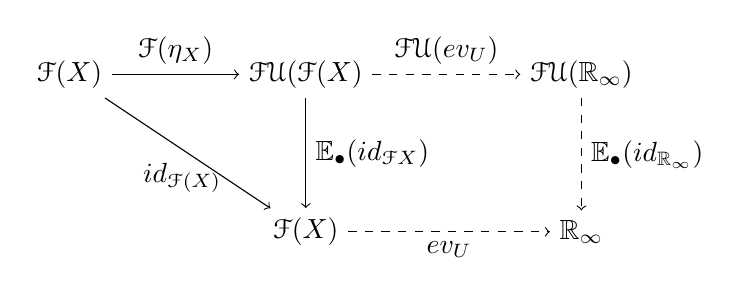
\begin{tikzpicture}
   \node  (FX)  at  (-1,0)  {$\mathcal{F}(X)$};
   \node  (FX2) at  (2,-2)  {$\mathcal{F}(X)$};
  \node  (FUFX) at  (2,0)  {$\mathcal{F}\mathcal{U}(\mathcal{F}(X)$};
  \node  (FUR)  at  (5.5,0)   {$\mathcal{F}\mathcal{U}(\Rinf)$};
  \node  (R)    at    (5.5, -2)  {$\Rinf$};

   \draw[->,above] (FX) to node {$\mathcal{F}(\eta_X)$} (FUFX);
  \draw[->,below] (FX) to node [xshift=-2pt]{$id_{\mathcal{F}(X)}$} (FX2);
  \draw[->,right] (FUFX) to node {$\mathbb{E}_{\bullet}(id_{\mathcal{F}X})$}  (FX2);
  \draw[->,above,dashed] (FUFX) to node {$\mathcal{F}\mathcal{U}(ev_U)$} (FUR);
  \draw[->,right,dashed] (FUR) to node {$\mathbb{E}_{\bullet}(id_{\Rinf})$} (R);
  \draw[->,below,dashed] (FX2) to node {$ev_U$} (R);
\end{tikzpicture}
\end{center}
commutes, i.e., $id_{\mathcal{F}(X)} = \mathbb{E}_{\bullet}(id_{\mathcal{F}(X)}) \circ \mathcal{F}(\eta_X)$.
Composition of those two parallel arrows by the affine measurable map $ev_U$, and using Lemma \ref{Lemma5} gives the commutative square on the right-hand side of the diagram.    Hence we seek to verify that the east-south path coincides with the diagonal-east path of the $\mathbf{Cvx}_{Meas}$-diagram.  Chasing elements we have, using $\delta_x(U)=\chi_U(x)$, 
\begin{center}
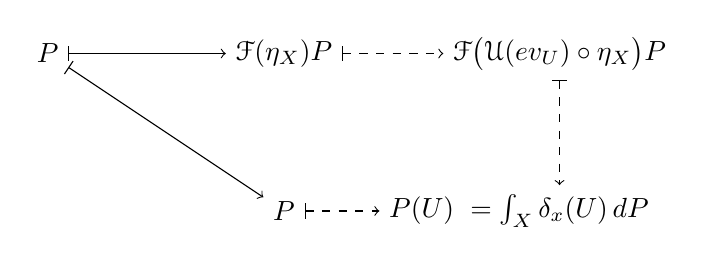
\begin{tikzpicture}
   \node  (FX)  at  (-1,0)  {$P$};
   \node  (FX2) at  (2,-2)  {$P$};
  \node  (FUFX) at  (2,0)  {$\mathcal{F}(\eta_X)P$};
  \node  (FUR)  at  (5.5,0)   {$\mathcal{F}\big(\mathcal{U}(ev_U) \circ \eta_X\big)P$};
  \node  (R)    at    (3.75, -2)  {$P(U)$};
  \node  (R2)    at    (5.5, -2)  {$=\int_X \delta_x(U) \, dP$};


   \draw[|->,above] (FX) to node {$$} (FUFX);
  \draw[|->,below] (FX) to node {} (FX2);
%  \draw[|->,right] (FUFX) to node {}  (FX2);
  \draw[|->,above,dashed] (FUFX) to node {} (FUR);
  \draw[|->,right,dashed] (FUR) to node {} (R2);
  \draw[|->,below,dashed] (FX2) to node {} (R);
\end{tikzpicture}
\end{center}
so $ev_U$ composed with both $id_{\mathcal{F}X}$ and $\mathbb{E}_{\bullet}(id_{\mathcal{F}(X)}) \circ \mathcal{F}(\eta_X)$ yield the same result.  This is true for every measurable set $U$ in $X$, and since the evaluation maps are jointly monic on $\mathcal{F}(X)$ it follows that the left triangle commutes.  Note that in this proof we have used the definition of a push forward probability measure to $\G(\Rinf)$, 
$$
\mathbb{E}_{\mathcal{F}\big( \mathcal{U}(ev_{\small{U}}) \circ \eta_X\big)P}(id_{\Rinf}) = \hat{\mathbb{E}}_P\big( \mathcal{U}(ev_{\tiny{U}}) \circ \eta_X\big).
$$
This is necessary to compute push forward probability measures by non-affine measurable functions $X \rightarrow \Rinf$.

To prove the second triangular equality let $A \in_{ob} \mathbf{Cvx}_{Meas}$.  We need to verify that the $\mathbf{Meas}$-diagram 
\begin{center}
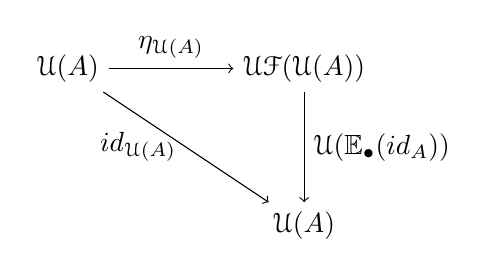
\begin{tikzpicture}
  \node  (UA) at  (0,0)  {$\mathcal{U}(A)$};
  \node  (UFUA) at  (3,0)  {$\mathcal{U}\mathcal{F}(\mathcal{U}(A))$};
  \node  (UA2)   at  (3, -2)  {$\mathcal{U}(A)$};
  \draw[->,above] (UA) to node {$\eta_{\mathcal{U}(A)}$} (UFUA);
  \draw[->,right] (UFUA) to node {$\mathcal{U}(\mathbb{E}_{\bullet}(id_A))$} (UA2);
  \draw[->,below,left] (UA) to node {$id_{\mathcal{U}(A)}$} (UA2);
\end{tikzpicture}
\end{center}
commutes.  Letting $a \in \mathcal{U}(A)$ we have
\begin{center}
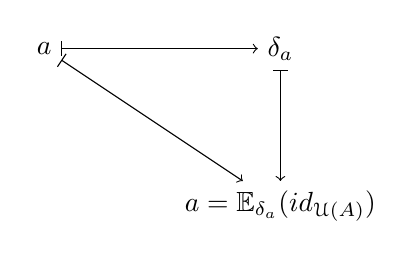
\begin{tikzpicture}
  \node  (UA) at  (0,0)  {$a$};
  \node  (UFUA) at  (3,0)  {$\delta_a$};
  \node  (UA2)   at  (3, -2)  {$a=\mathbb{E}_{\delta_a}(id_{\mathcal{U}(A)})$};
  \draw[|->,above] (UA) to node {} (UFUA);
  \draw[|->,right] (UFUA) to node {} (UA2);
  \draw[|->,below,left] (UA) to node {} (UA2);
\end{tikzpicture}
\end{center}
which proves the second triangular equality, and we conclude $\langle \mathcal{F}, \mathcal{U}, \eta, \mathbb{E} \rangle$ forms an adjunction.

We now proceed to show the adjunction yields the Giry monad.  It is clear that $\G = \mathcal{U} \circ \mathcal{F}$, and we have essentially already shown in the proof of Lemma 6 that $\mu_X = \mathcal{U}\big(\mathbb{E}_{\bullet}(id_{\mathcal{F}(X)})$.  We need only to alter equation (14) by replacing the term $\mathbb{E}_{\bullet}(id_{\G(X)})$ with the term $\mathbb{E}_{\bullet}(id_{\F(X)})$ which is valid because the functor $\F$ is the functor $\G$ viewed as a functor into $\mathbf{Cvx}_{Meas}$.
\end{proof}

\end{document}
